\section{Results} % min 7 pages
\label{sec:results}

%%%%%%%%%%%%%%%%%%%%%%%%%%%%%%%%%%%%%%%%%%%%%%%%%%%%%%%%%%%%%%%%%%%%%%%%%%%%%%%%%%%%%%%%%%%%%%%
%%%%%%%%% PDFs
%%%%%%%%%%%%%%%%%%%%%%%%%%%%%%%%%%%%%%%%%%%%%%%%%%%%%%%%%%%%%%%%%%%%%%%%%%%%%%%%%%%%%%%%%%%%%%%
\begin{figure}
\hfill
\begin{minipage}{.45\linewidth}
	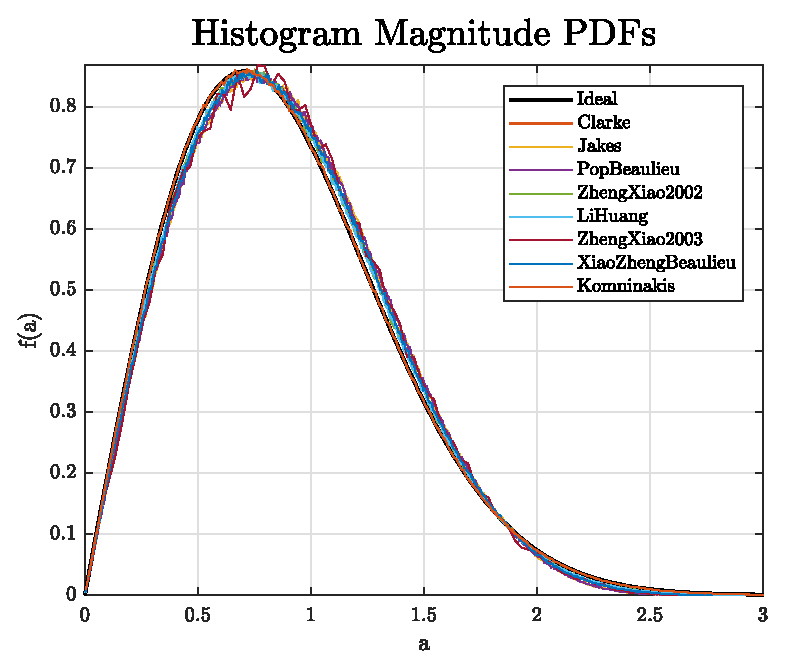
\includegraphics[width=\linewidth]{img/histMag.eps}
\end{minipage}
\hfill
\begin{minipage}{.45\linewidth}
	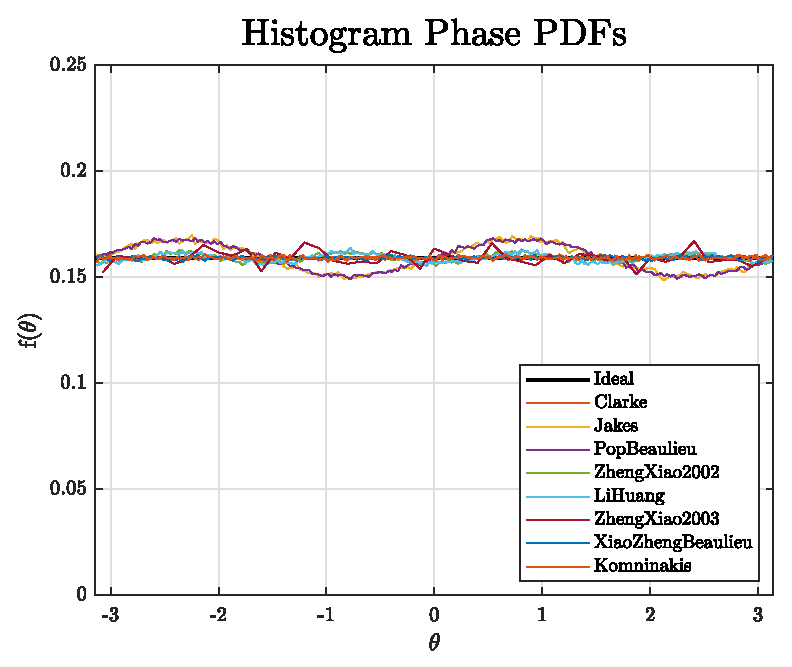
\includegraphics[width=\linewidth]{img/histPhase.eps}
\end{minipage}
\hfill

\caption{Histograms of Magnitudes and Phases of all the implemented simulators. Note the aforementioned problem with ZhengXiao2003}
\label{fig:histograms}
\end{figure}

Note that ZhengXiao2003 has a particularly zigzagy line since the first few samples did not respect the distributions. Computing more samples, then, didn't allow me to create as many channels as for the others due to memory limitations.

%%%%%%%%%%%%%%%%%%%%%%%%%%%%%%%%%%%%%%%%%%%%%%%%%%%%%%%%%%%%%%%%%%%%%%%%%%%%%%%%%%%%%%%%%%%%%%%
%%%%%%%%%%%% Correlations
%%%%%%%%%%%%%%%%%%%%%%%%%%%%%%%%%%%%%%%%%%%%%%%%%%%%%%%%%%%%%%%%%%%%%%%%%%%%%%%%%%%%%%%%%%%%%%%

\begin{figure}
	\hfill
	\begin{minipage}{.45\linewidth}
		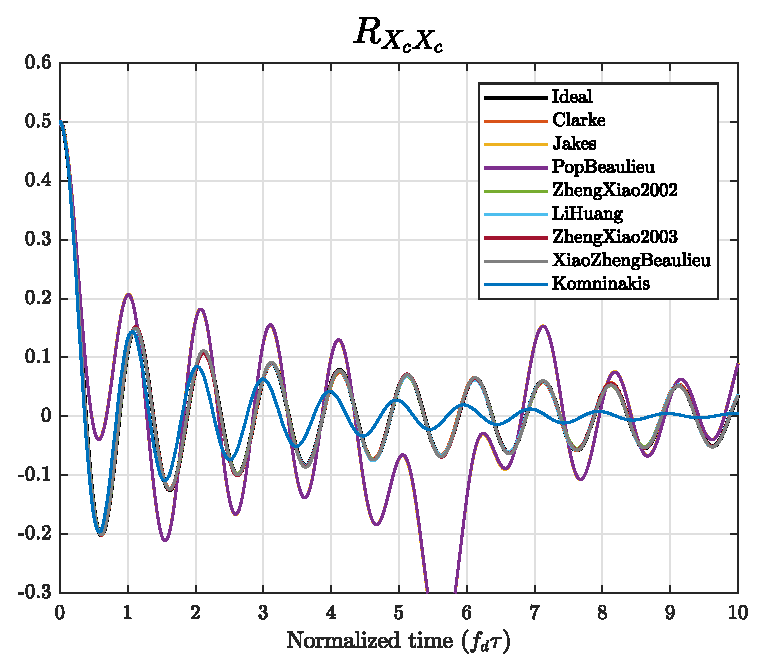
\includegraphics[width=\linewidth]{img/XcXc.eps}
	\end{minipage}
	\hfill
	\begin{minipage}{.45\linewidth}
		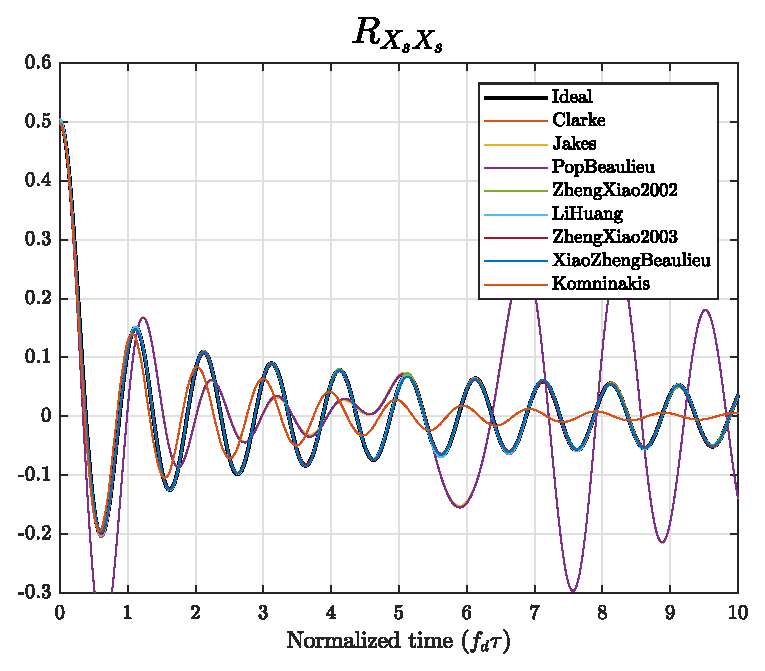
\includegraphics[width=\linewidth]{img/XsXs.eps}
	\end{minipage}
	\hfill
	
	\vspace{2mm}
	
	\hfill
	\begin{minipage}{.45\linewidth}
		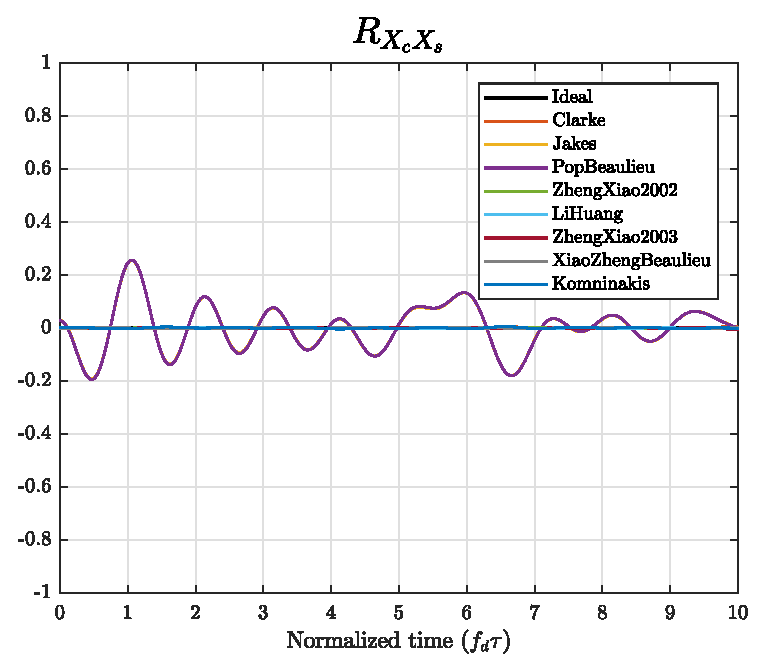
\includegraphics[width=\linewidth]{img/XcXs.eps}
	\end{minipage}
	\hfill
	\begin{minipage}{.45\linewidth}
		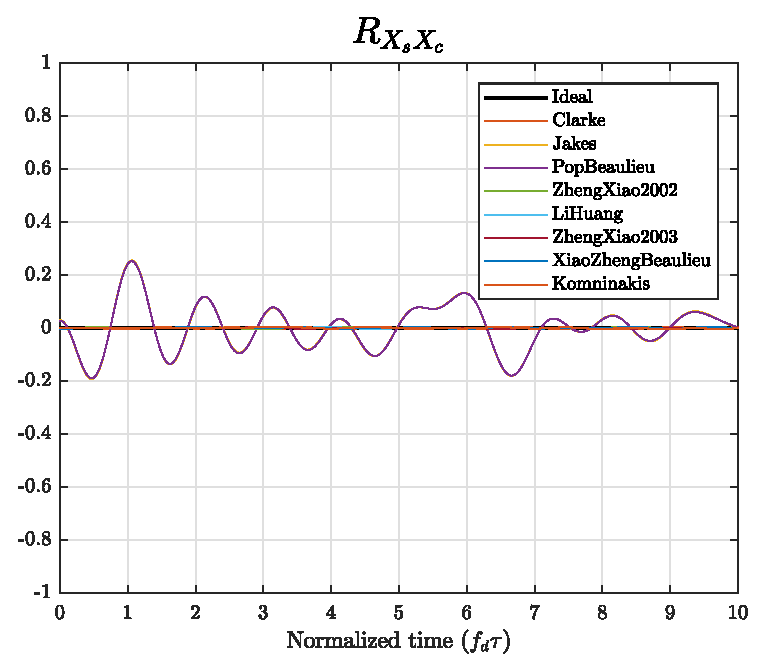
\includegraphics[width=\linewidth]{img/XsXc.eps}
	\end{minipage}
	\hfill
	
	\caption{Cross correlations between real and imaginary components}
	\label{fig:4xcorr}
\end{figure}

\begin{figure}
	\hfill
	\begin{minipage}{.32\linewidth}
		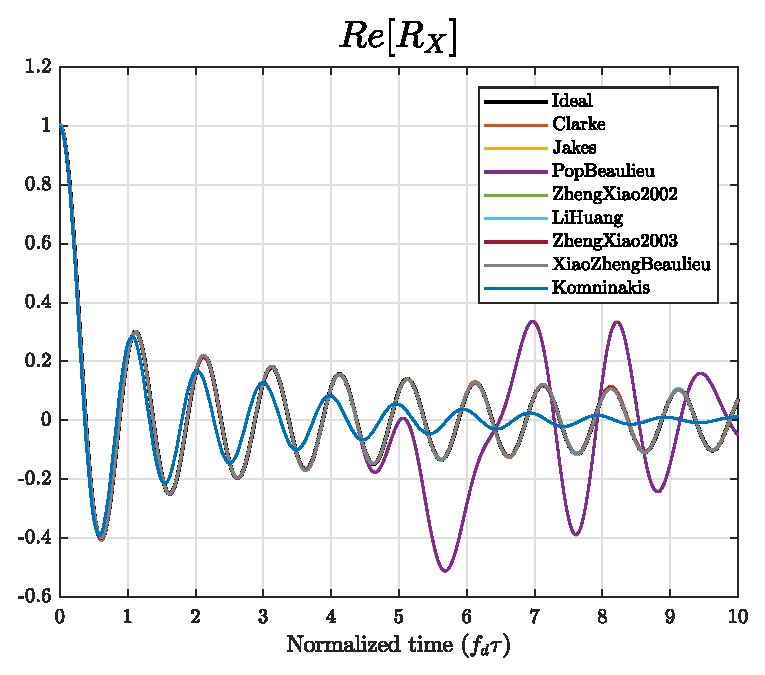
\includegraphics[width=\linewidth]{img/ReX.eps}
	\end{minipage}
	\hfill
	\begin{minipage}{.32\linewidth}
		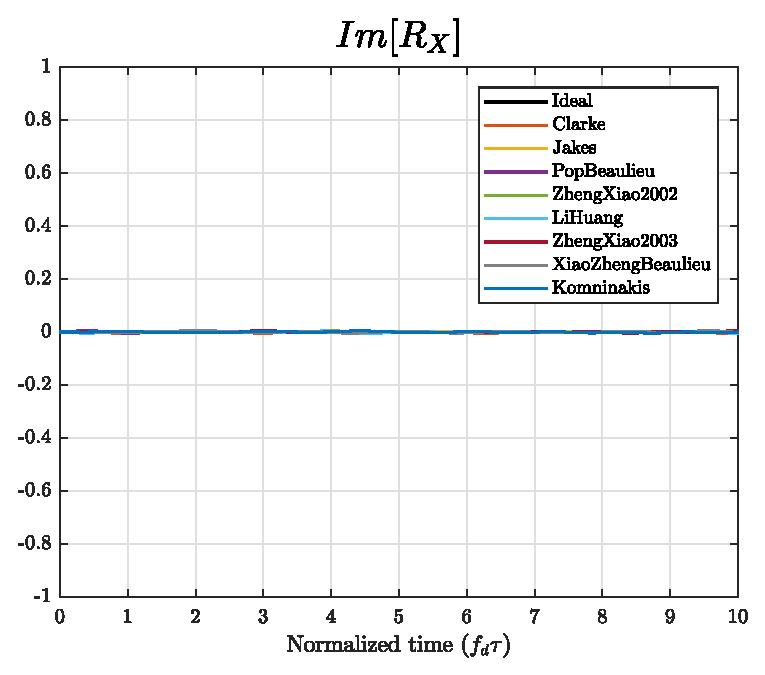
\includegraphics[width=\linewidth]{img/ImX.eps}
	\end{minipage}
	\hfill
	\begin{minipage}{.32\linewidth}
		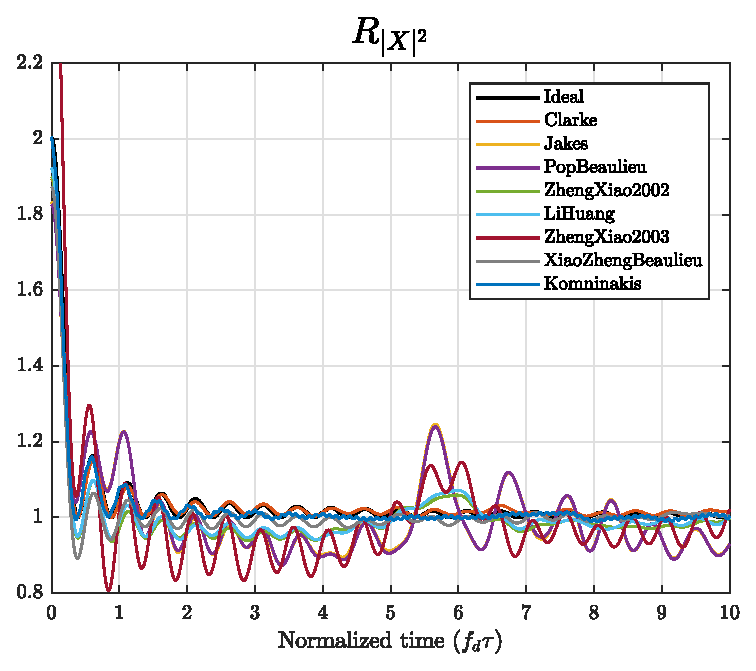
\includegraphics[width=\linewidth]{img/X2.eps}
	\end{minipage}
	\hfill
	
	\caption{Correlations of the channels}
	\label{fig:3xcorr}
\end{figure}

%%%%%%%%%%%%%%%%%%%%%%%%%%%%%%%%%%%%%%%%%%%%%%%%%%%%%%%%%%%%%%%%%%%%%%%%%%%%%%%%%%%%%%%%%%%%%%%
%%%%%%%%%%%% LCR/AFD
%%%%%%%%%%%%%%%%%%%%%%%%%%%%%%%%%%%%%%%%%%%%%%%%%%%%%%%%%%%%%%%%%%%%%%%%%%%%%%%%%%%%%%%%%%%%%%%
\begin{figure}
	\hfill
	\begin{minipage}{.45\linewidth}
		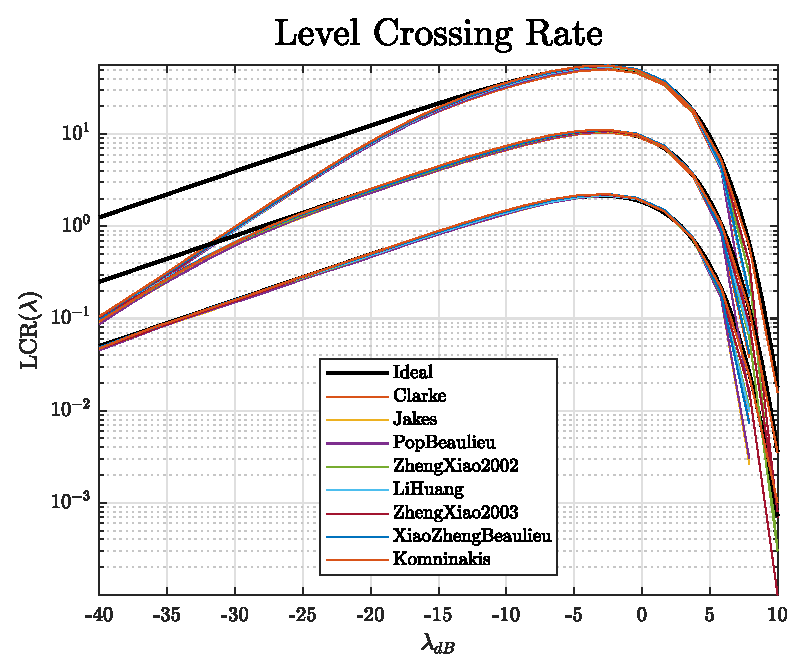
\includegraphics[width=\linewidth]{img/multiLCR.eps}
	\end{minipage}
	\hfill
	\begin{minipage}{.45\linewidth}
		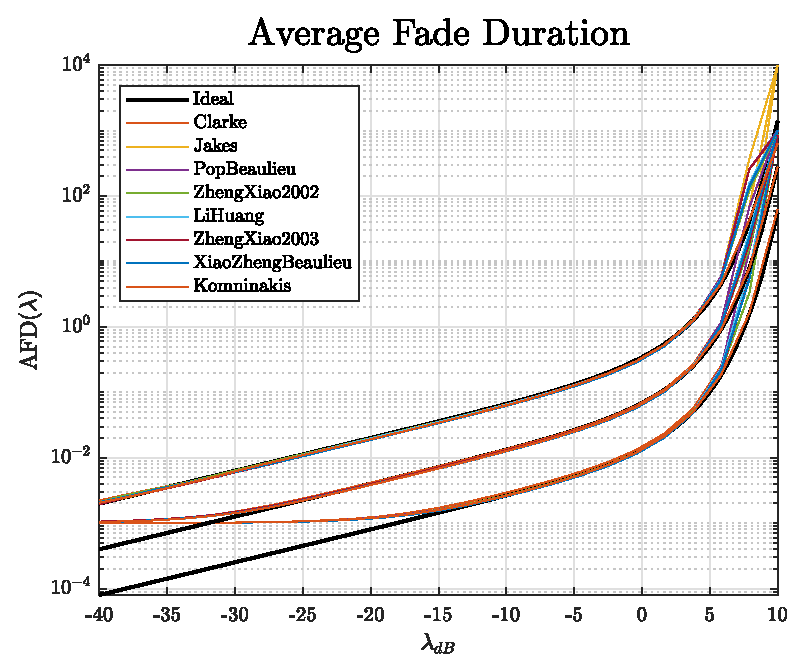
\includegraphics[width=\linewidth]{img/multiAFD.eps}
	\end{minipage}
	\hfill
	
	\caption{Plots for threshold-based statistics. Note that $\lambda_{dB} \triangleq 20\, \log_{10} \lambda$ since it's envelope related, not power related}
	\label{fig:LCR_AFD}
\end{figure}

%%%%%%%%%%%%%%%%%%%%%%%%%%%%%%%%%%%%%%%%%%%%%%%%%%%%%%%%%%%%%%%%%%%%%%%%%%%%%%%%%%%%%%%%%%%%%%%
%%%%%%%%%%%% Simulation Time
%%%%%%%%%%%%%%%%%%%%%%%%%%%%%%%%%%%%%%%%%%%%%%%%%%%%%%%%%%%%%%%%%%%%%%%%%%%%%%%%%%%%%%%%%%%%%%%
\begin{figure}
	\hfill
	\subfigure[Overall Simulation Time]{
		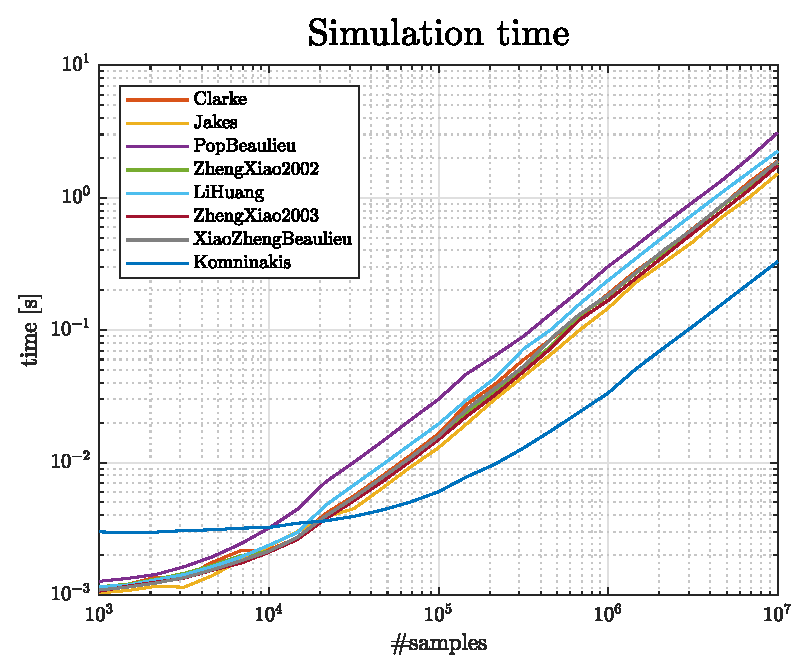
\includegraphics[width=.31\linewidth]{img/simTime.eps}
	}
	\hfill
	\subfigure[Kominakis Simulation Time]{
		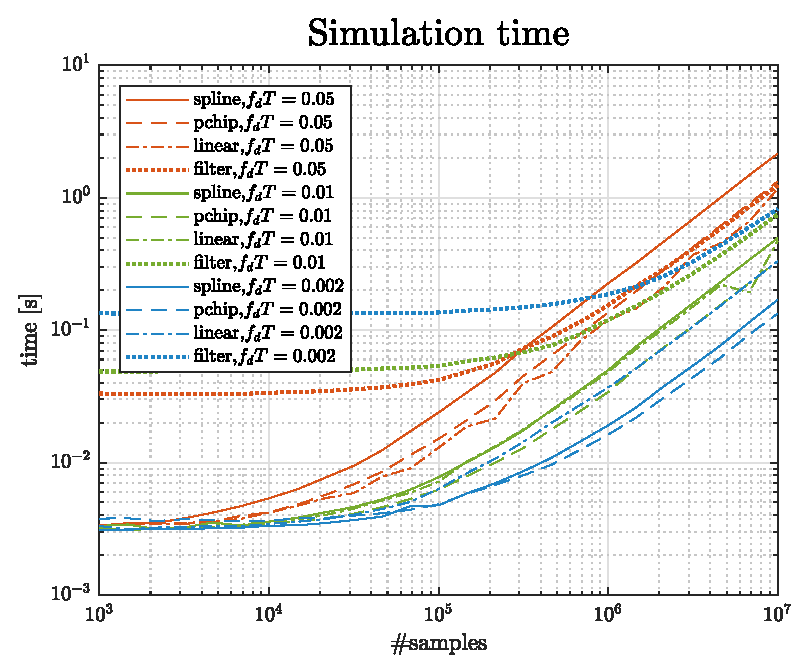
\includegraphics[width=.31\linewidth]{img/simTime_Komninakis.eps}
	}
	\hfill
	\subfigure[Simulation Time for different $N_{ch}$]{
		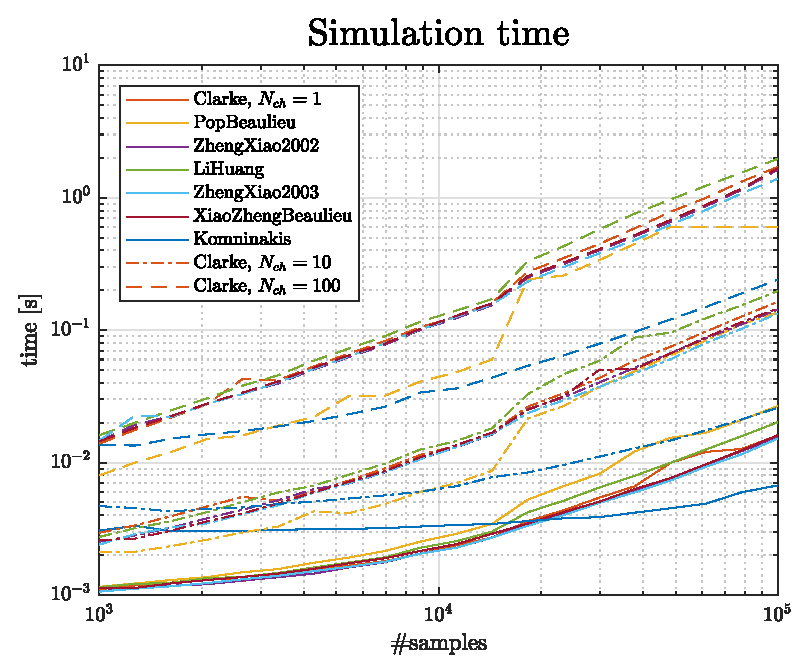
\includegraphics[width=.31\linewidth]{img/multiSimTime.eps}
	}
	\hfill
	
	\caption{Simulation time for current implementations}
	\label{fig:simTime}
\end{figure}